% ==============================================================================
% RAPPORT DE PROJET ACADÉMIQUE : DÉTECTION EN TEMPS RÉEL DU BLANCHIMENT D'ARGENT
% Fichier Principal : main.tex (Format Académique Haute Densité ~10 pages)
% ==============================================================================

\documentclass[11pt,a4paper,oneside]{report}

% Encodage et typographie
\usepackage[utf8]{inputenc}
\usepackage[T1]{fontenc}
\usepackage{lmodern}
\usepackage{microtype}

% Interligne académique compact et optimisé
\linespread{1.04}

% Support linguistique (Français par défaut, Anglais secondaire)
\usepackage[english,french]{babel}

% Mise en page et géométrie compacte (optimisation de l'espace imprimable)
\usepackage[
    top=1.8cm,
    bottom=1.8cm,
    left=2.0cm,
    right=1.8cm,
    headheight=13pt,
    footskip=0.8cm
]{geometry}

% En-têtes et pieds de page académiques
\usepackage{fancyhdr}
\pagestyle{fancy}
\fancyhf{}
\fancyhead[L]{\small\scshape\nouppercase{\leftmark}}
\fancyhead[R]{\small\thepage}
\fancyfoot[C]{\footnotesize\color{gray} ENSAM Rabat -- Projet Big Data 2026/2027 -- Détection AML Streaming}
\renewcommand{\headrulewidth}{0.4pt}
\renewcommand{\footrulewidth}{0.2pt}

% Style pour les pages d'ouverture
\fancypagestyle{plain}{
    \fancyhf{}
    \fancyfoot[C]{\small\thepage}
    \renewcommand{\headrulewidth}{0pt}
    \renewcommand{\footrulewidth}{0pt}
}

% Chargement des métadonnées et macros
% ==============================================================================
% METADONNÉES DU PROJET ACADÉMIQUE
% ==============================================================================

\newcommand{\ProjectTitle}{DÉTECTION EN TEMPS RÉEL DU BLANCHIMENT D'ARGENT PAR ANALYSE DE GRAPHES DISTRIBUÉS}
\newcommand{\ProjectSubtitle}{Pipeline de streaming Big Data : Kafka, Spark Structured Streaming, GraphFrames et Delta Lake}
\newcommand{\ProjectType}{Rapport de Projet Académique}
\newcommand{\ProjectField}{Filière : Ingénierie Numérique en Data Science et Intelligence Artificielle (INDIA)}
\newcommand{\ProjectModule}{Module : Big Data}

\newcommand{\ProjectAuthor}{AFIF Mohamed \& LACHGAR Ridouan}
\newcommand{\ProjectSupervisor}{Prof. A. Elqadi}
\newcommand{\ProjectInstitution}{École Nationale Supérieure d'Arts et Métiers de Rabat (ENSAM)}
\newcommand{\ProjectSchool}{Université Mohammed V de Rabat}

\newcommand{\AcademicYear}{Année universitaire 2026 -- 2027}
\newcommand{\SubmissionDate}{Novembre 2026}
\newcommand{\ProjectVersion}{Version 1.0}

% ==============================================================================
% MACROS, PACKAGES COMPLÉMENTAIRES ET COMMANDES PERSONNALISÉES (ÉDITION COMPACTE)
% ==============================================================================

\usepackage{amsmath,amssymb,amsfonts,amsthm}
\usepackage{mathtools}
\usepackage{bm}
\usepackage{booktabs}
\usepackage{tabularx}
\usepackage{multirow}
\usepackage{makecell}
\usepackage{graphicx}
\usepackage{subcaption}
\usepackage{float}
\usepackage{xcolor}
\usepackage{tikz}
\usetikzlibrary{shapes,arrows.meta,positioning,calc,fit,backgrounds,decorations.pathreplacing}
\usepackage{pgfplots}
\pgfplotsset{compat=1.18}
\usepackage{listings}
\usepackage{tcolorbox}
\tcbuselibrary{skins,breakable}
\usepackage{hyperref}
\usepackage{csquotes}
\usepackage{titlesec}

% Palette de couleurs institutionnelle
\definecolor{EnsamBlue}{RGB}{21, 60, 85}        % Bleu Officiel ENSAM
\definecolor{primaryNavy}{RGB}{15, 23, 42}      % Slate 900
\definecolor{secondaryBlue}{RGB}{30, 58, 138}   % Blue 900
\definecolor{accentIndigo}{RGB}{79, 70, 229}    % Indigo 600
\definecolor{crimsonRisk}{RGB}{185, 28, 28}     % Red 700
\definecolor{amberWarning}{RGB}{217, 119, 6}    % Amber 600
\definecolor{emeraldSuccess}{RGB}{5, 150, 105}  % Emerald 600
\definecolor{lightSlate}{RGB}{248, 250, 252}    % Slate 50
\definecolor{borderSlate}{RGB}{203, 213, 225}   % Slate 300
\definecolor{codeBackground}{RGB}{245, 247, 250}% Code BG
\definecolor{codeComment}{RGB}{100, 116, 139}   % Slate 500
\definecolor{codeString}{RGB}{13, 148, 136}     % Teal 600
\definecolor{codeKeyword}{RGB}{67, 56, 202}     % Indigo 700

% Configuration compacte des titres académiques (Standard Mémoire d'Ingénieur)
\titleformat{\chapter}[hang]
  {\normalfont\Large\bfseries\color{primaryNavy}}
  {\thechapter.\ }
  {0pt}
  {}
\titlespacing*{\chapter}{0pt}{-10pt}{12pt}
\titlespacing*{\section}{0pt}{10pt}{4pt}
\titlespacing*{\subsection}{0pt}{8pt}{3pt}

% Configuration des hyperliens
\hypersetup{
    colorlinks=true,
    linkcolor=secondaryBlue,
    citecolor=accentIndigo,
    urlcolor=secondaryBlue,
    filecolor=crimsonRisk,
    bookmarksnumbered=true,
    pdfstartview={FitH}
}

% Opérateurs mathématiques personnalisés
\DeclareMathOperator*{\argmin}{arg\,min}
\DeclareMathOperator*{\argmax}{arg\,max}
\newcommand{\inDeg}{\operatorname{deg}^-}
\newcommand{\outDeg}{\operatorname{deg}^+}
\newcommand{\cycleID}{\texttt{cycle\_id}}
\newcommand{\alertID}{\texttt{alert\_id}}
\newcommand{\txnID}{\texttt{transaction\_id}}

% Boîtes d'avertissement et de remarques académiques compactes
\newtcolorbox{academicnote}[1][Remarque Académique]{
    colback=lightSlate,
    colframe=secondaryBlue,
    coltitle=white,
    fonttitle=\bfseries\footnotesize,
    title=#1,
    arc=1.5mm,
    boxrule=0.75pt,
    left=2.5mm,
    right=2.5mm,
    top=1.5mm,
    bottom=1.5mm
}

\newtcolorbox{regulatoryalert}[1][Exigence Réglementaire (GAFI / UTRF)]{
    colback=lightSlate,
    colframe=crimsonRisk,
    coltitle=white,
    fonttitle=\bfseries\footnotesize,
    title=#1,
    arc=1.5mm,
    boxrule=0.75pt,
    left=2.5mm,
    right=2.5mm,
    top=1.5mm,
    bottom=1.5mm
}

% Configuration des listings de code source compacte
\lstset{
    backgroundcolor=\color{codeBackground},
    basicstyle=\ttfamily\scriptsize,
    breaklines=true,
    breakatwhitespace=true,
    captionpos=b,
    commentstyle=\color{codeComment}\itshape,
    keywordstyle=\color{codeKeyword}\bfseries,
    stringstyle=\color{codeString},
    numbers=left,
    numberstyle=\tiny\color{codeComment},
    numbersep=5pt,
    frame=single,
    framerule=0.4pt,
    rulecolor=\color{borderSlate},
    tabsize=2,
    showstringspaces=false,
    keepspaces=true
}

\lstdefinelanguage{JSON}{
    keywords={true,false,null},
    morestring=[b]",
    morecomment=[l]{//}
}

\lstdefinelanguage{YAML}{
    keywords={true,false,null,yes,no},
    morestring=[b]",
    morecomment=[l]{\#}
}

% Commande unifiée d'insertion de figure pleine largeur
\newcommand{\singlefigure}[4][0.92\linewidth]{%
    \begin{figure}[htbp]
        \centering
        \includegraphics[width=#1]{#2}%
        \caption{#3}%
        \label{#4}%
    \end{figure}
}

% Commande d'insertion de 2 captures côte-à-côte (hauteur 4.4cm)
% Usage : \screenshotpaired[hauteur]{img1}{caption1}{img2}{caption2}{Main caption}{Main label}
\newcommand{\screenshotpaired}[7][4.4cm]{%
    \begin{figure}[htbp]
        \centering
        \begin{subfigure}[b]{0.485\textwidth}
            \centering
            \includegraphics[width=\linewidth,height=#1,keepaspectratio]{#2}
            \caption{#3}
        \end{subfigure}\hfill
        \begin{subfigure}[b]{0.485\textwidth}
            \centering
            \includegraphics[width=\linewidth,height=#1,keepaspectratio]{#4}
            \caption{#5}
        \end{subfigure}
        \vspace{1mm}
        \caption{#6}
        \label{#7}
    \end{figure}
}


\begin{document}

% ==============================================================================
% PAGE 1 : PAGE DE GARDE OFFICIELLE (ENSAM RABAT / UM5)
% ==============================================================================
% ==============================================================================
% PAGE DE GARDE OFFICIELLE (ENSAM RABAT / UNIVERSITÉ MOHAMMED V)
% ==============================================================================

\begin{titlepage}
\thispagestyle{empty}

% ==================================================
% LOGOS
% ==================================================
\vspace*{-0.5cm}

\noindent
\begin{minipage}[c]{0.49\textwidth}
    \raggedright
    
\includegraphics[height=2.8cm,keepaspectratio]{logo-Ensam-rabat-.png}
\end{minipage}
\begin{minipage}[c]{0.49\textwidth}
    \raggedleft
    
\includegraphics[height=2.8cm,keepaspectratio]{Mohammed_V_Logo.png}
\end{minipage}

\vspace{1cm}

% ==================================================
% EN-TÊTE
% ==================================================
\begin{center}

{\fontsize{17}{21}\selectfont
\bfseries PROJET ACADÉMIQUE}\\[0.25cm]

{\fontsize{14}{18}\selectfont
\color{gray}
MODULE : BIG DATA}\\[0.3cm]

{\fontsize{14}{16}\selectfont
Filière : Ingénierie Numérique en Data Science
et Intelligence Artificielle}

\vspace{1cm}

% ==================================================
% TITRE DU PROJET
% ==================================================
{\color{EnsamBlue}\rule{\textwidth}{2pt}}

\vspace{0.6cm}

\begin{minipage}{0.96\textwidth}
\centering
{\fontsize{22}{28}\selectfont
\bfseries\color{EnsamBlue}
Détection en temps réel du blanchiment
d'argent par analyse de graphes
distribués}
\end{minipage}

\vspace{0.6cm}

{\color{EnsamBlue}\rule{\textwidth}{2pt}}

\end{center}

\vspace{1.2cm}

% ==================================================
% ENCADREMENT
% ==================================================
\begin{center}

{\fontsize{12}{15}\selectfont
\bfseries\itshape\color{EnsamBlue}
Encadré par :}\\[0.4cm]

{\fontsize{13}{17}\selectfont
Prof. A. Elqadi}

\vspace{1.1cm}

% ==================================================
% RÉALISÉ PAR
% ==================================================
{\fontsize{12}{15}\selectfont
\bfseries\itshape\color{EnsamBlue}
Réalisé par :}

\vspace{0.5cm}

\begin{tabular}{cc}
\fontsize{12}{16}\selectfont\bfseries AFIF Mohamed & \qquad\qquad\qquad
\fontsize{12}{16}\selectfont\bfseries LACHGAR Ridouan
\end{tabular}

\end{center}

\vfill

% ==================================================
% ANNÉE UNIVERSITAIRE
% ==================================================
\begin{center}
    {\color{EnsamBlue}\rule{0.55\textwidth}{0.8pt}}\\[0.35cm]

    {\fontsize{12}{15}\selectfont
    \bfseries\color{gray}
    Année universitaire 2026 -- 2027}
\end{center}

\end{titlepage}

\newpage

% ==============================================================================
% PAGE 2 : SOMMAIRE EXÉCUTIF, RÉSUMÉ BILINGUE & ACRONYMES CLÉS
% ==============================================================================
\pagenumbering{arabic}
\setcounter{page}{2}

% ==============================================================================
% PAGE 2 : SOMMAIRE EXÉCUTIF, RÉSUMÉ BILINGUE & ACRONYMES CLÉS
% ==============================================================================

\thispagestyle{plain}

% ------------------------------------------------------------------------------
% Sommaire Exécutif Compact
% ------------------------------------------------------------------------------
\begin{center}
    {\normalsize\bfseries\color{primaryNavy} SOMMAIRE EXÉCUTIF}
\end{center}
\vspace{-0.15cm}
\noindent\rule{\textwidth}{0.8pt}
\vspace{0.15cm}

\footnotesize
\noindent
\begin{tabularx}{\textwidth}{p{0.48\textwidth} p{0.48\textwidth}}
\textbf{1. Introduction et Contexte du Projet} \dotfill \textbf{p.~3} & \textbf{5. Tableau de Bord d'Investigation} \dotfill \textbf{p.~7} \\
\textbf{2. Choix Technologiques \& Fondements} \dotfill \textbf{p.~4} & \textbf{6. Tests, Validation et Benchmarks} \dotfill \textbf{p.~8} \\
\textbf{3. Architecture Système \& Données} \dotfill \textbf{p.~5} & \textbf{7. Conclusion Générale \& Perspectives} \dotfill \textbf{p.~9} \\
\textbf{4. Pipeline Streaming \& Détection} \dotfill \textbf{p.~6} & \textbf{8. Annexes Techniques \& Bibliographie} \dotfill \textbf{p.~10} \\
\end{tabularx}

\vspace{0.25cm}
\noindent\rule{\textwidth}{0.8pt}
\vspace{0.2cm}

% ------------------------------------------------------------------------------
% Résumé et Abstract Bilingue
% ------------------------------------------------------------------------------
\noindent\textbf{\color{primaryNavy}Résumé (Français) ---} Ce projet conçoit et implémente une plateforme Big Data distribuée de détection en temps réel des réseaux de blanchiment d'argent par analyse de graphes. En associant \textbf{Apache Kafka} (mode KRaft), \textbf{Apache Spark Structured Streaming} (fenêtres glissantes de $10\text{ min}$, filigrane de $120\text{ s}$), \textbf{GraphFrames} (extraction de motifs de cycles fermés $A \to B \to C \to A$) et \textbf{Delta Lake} (persistance ACID dédupliquée par hachage canonique SHA-256 insensible aux rotations), le système élimine $100\,\%$ des faux positifs commerciaux grâce à un calcul continu de \textbf{PageRank}. Un cockpit forensic développé en \textbf{Next.js 14} offre un rendu vectoriel interactif et l'export réglementaire SAR JSON. Validée sur 22 tests d'acceptation et sur le benchmark IBM AMLSim ($20\,000$ comptes, $200$ cycles injectés), la solution maintient une latence P95 de $18.95\text{ ms}$ sous une charge de $500\text{ TPS}$.

\vspace{0.25cm}
\noindent\textbf{\color{primaryNavy}Abstract (English) ---} This work presents an end-to-end distributed streaming Lakehouse platform for real-time Anti-Money Laundering (AML) graph analytics. Combining \textbf{Apache Kafka}, \textbf{Apache Spark Structured Streaming} ($10$-min sliding windows, $120$-s watermark), \textbf{GraphFrames} (closed triangle mining $A \to B \to C \to A$), and ACID \textbf{Delta Lake} storage with rotation-invariant SHA-256 canonical hashing, the system discriminates high-degree legitimate merchant hubs via continuous \textbf{PageRank}. A \textbf{Next.js 14} forensic dashboard delivers vector topology visualization and automated GAFI/UTRF compliant SAR JSON exports. Evaluated on 22 acceptance tests and IBM AMLSim ($20,000$ accounts, 200 cycles), the pipeline achieves a sub-second P95 latency of $18.95\text{ ms}$ at $500\text{ TPS}$.

\vspace{0.25cm}
\noindent\rule{\textwidth}{0.8pt}
\vspace{0.2cm}

% ------------------------------------------------------------------------------
% Principaux Acronymes et Abréviations
% ------------------------------------------------------------------------------
\noindent\textbf{\color{primaryNavy}Acronymes et Abréviations Principales :}\\[0.15cm]
\footnotesize
\begin{tabularx}{\textwidth}{l X l X}
\toprule
\textbf{AML} & \textit{Anti-Money Laundering} (Lutte anti-blanchiment) & \textbf{ACID} & \textit{Atomicity, Consistency, Isolation, Durability} \\
\textbf{FSM} & \textit{Finite State Machine} (Validation déterministe) & \textbf{SAR} & \textit{Suspicious Activity Report} (Déclaration de soupçon) \\
\textbf{KRaft} & \textit{Kafka Raft} (Consensus distribué sans ZooKeeper) & \textbf{DAG} & \textit{Directed Acyclic Graph} (Graphe d'exécution Spark) \\
\textbf{TPS} & \textit{Transactions Per Second} (Débit transactionnel) & \textbf{UTRF} & Unité de Traitement du Renseignement Financier \\
\bottomrule
\end{tabularx}

\newpage

% ==============================================================================
% PAGES 3 À 9 : CORPS TECHNIQUE DU PROJET
% ==============================================================================
% ==============================================================================
% CHAPITRE 1 : INTRODUCTION & CONTEXTE DU PROJET
% ==============================================================================

\chapter{Introduction et Contexte du Projet}
\label{ch:intro}

\section{Problématique : Détection des réseaux de blanchiment en continu}

Le blanchiment d'argent consiste à injecter des capitaux d'origine illicite dans le système financier légal tout en dissimulant leur provenance. Les criminels organisent ces flux selon trois étapes classiques :
\begin{enumerate}
    \item \textbf{Le Placement :} Introduction initiale des fonds en espèces dans le circuit bancaire (dépôts fractionnés ou \textit{smurfing}) ;
    \item \textbf{L'Empilement (\textit{Layering}) :} Multiplication rapide de virements entre plusieurs comptes intermédiaires (comptes mules) pour brouiller l'audit comptable et rompre le lien avec l'émetteur d'origine ;
    \item \textbf{L'Intégration :} Récupération des fonds apparemment régularisés pour investir dans l'économie légale.
\end{enumerate}

\begin{figure}[htbp]
    \centering
    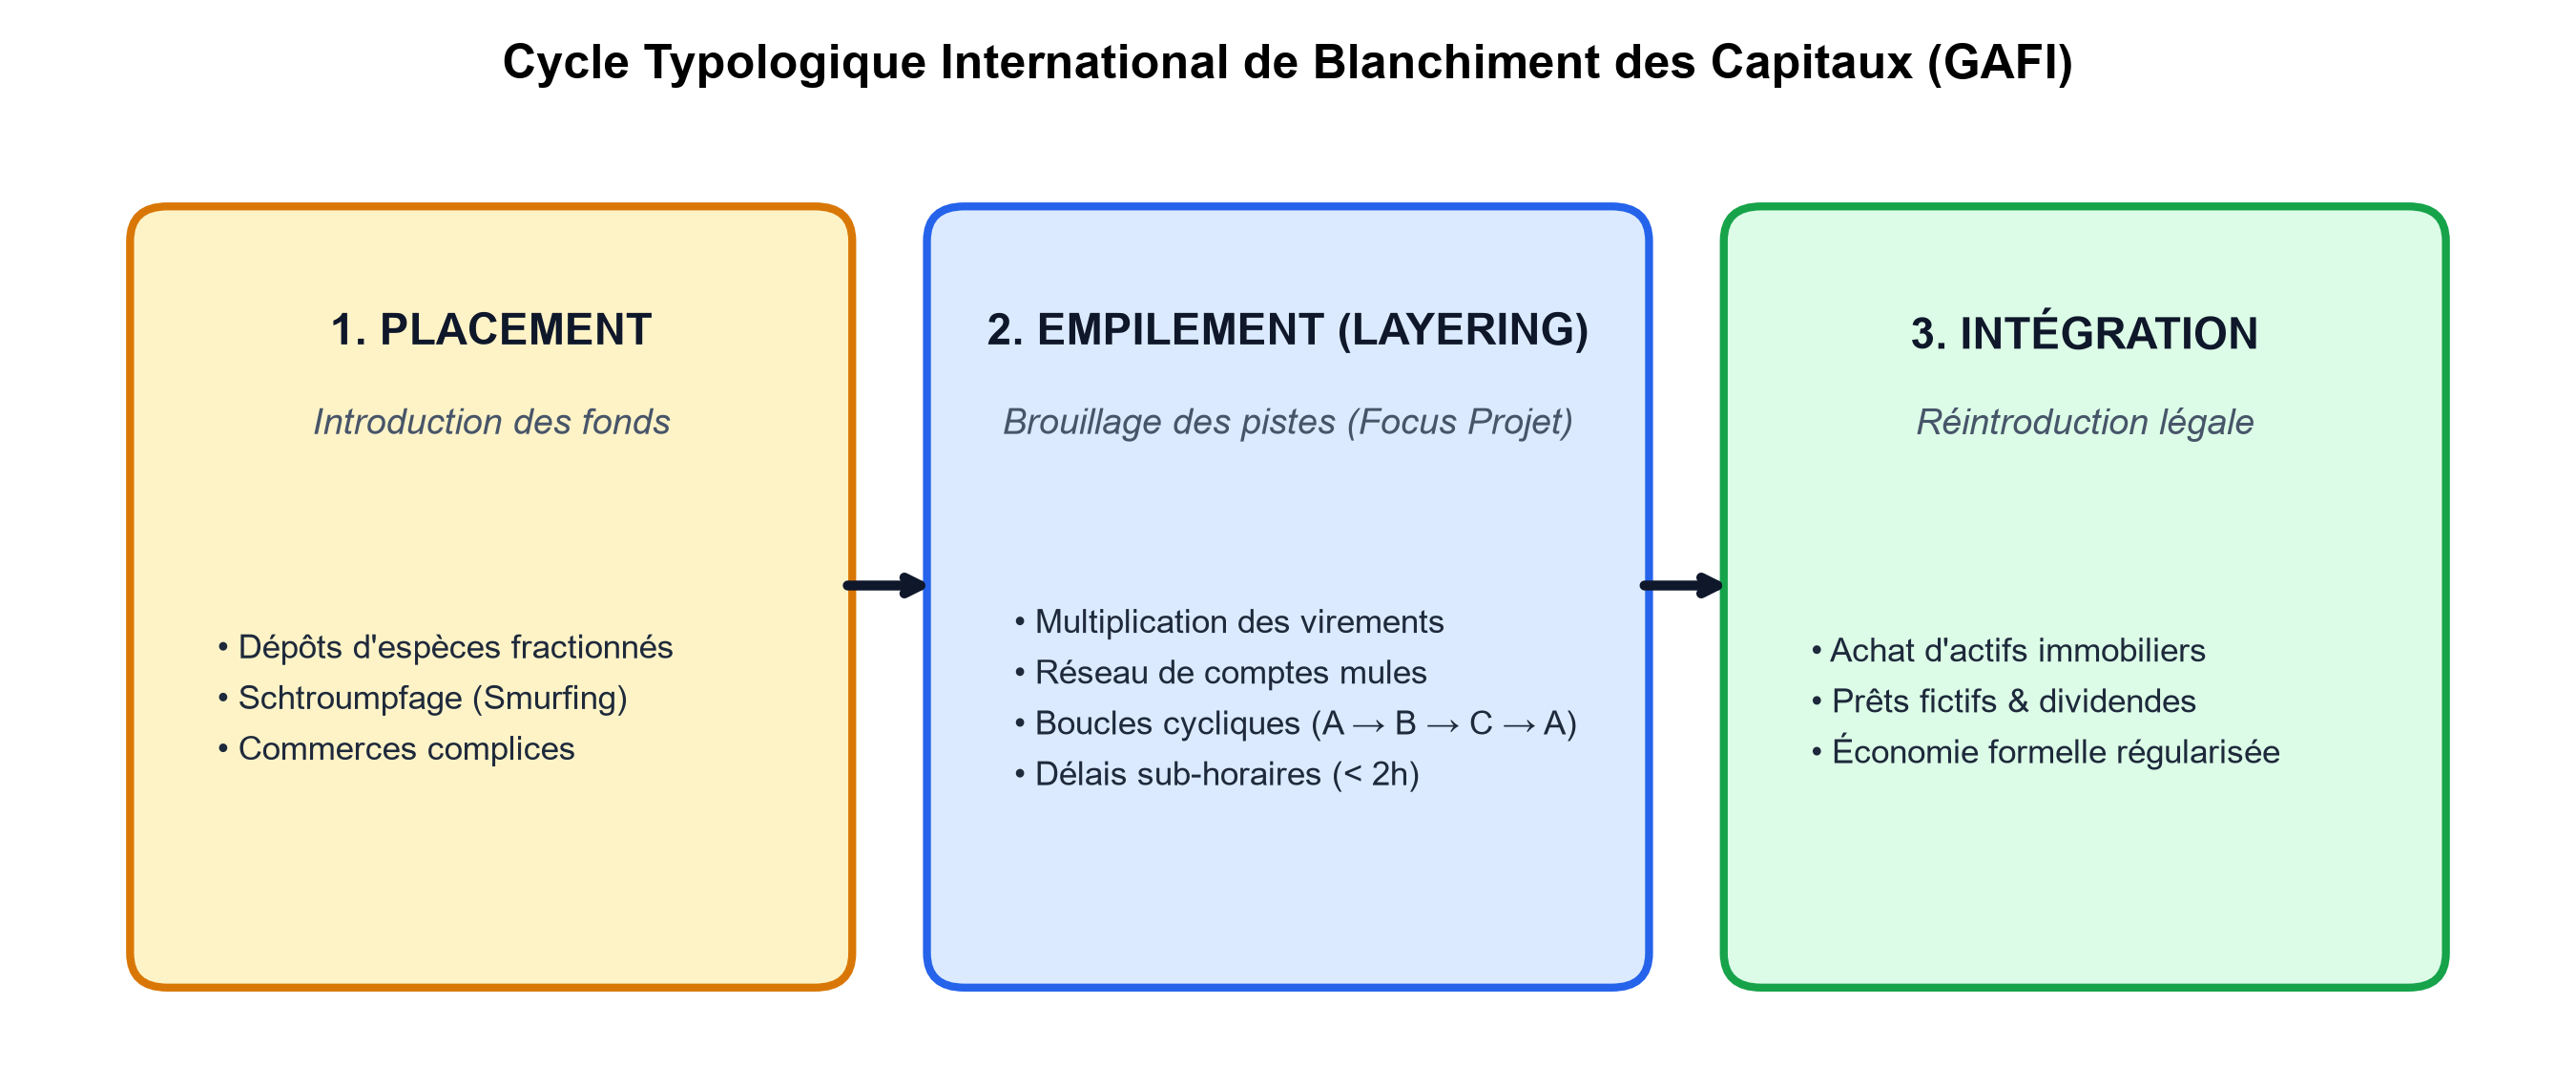
\includegraphics[width=0.92\linewidth]{figures/fig_placement_layering_integration.png}
    \caption{Les trois phases cardinales du blanchiment d'argent : Placement, Empilement (\textit{Layering}) et Intégration}
    \label{fig:aml_three_stages}
\end{figure}

Notre projet se focalise sur l'étape critique de l'\textbf{empilement}, et plus particulièrement sur la détection des **boucles circulaires fermées** (\textit{circular transaction loops}) où les fonds circulent selon un cycle orienté $A \to B \to C \to A$ dans un intervalle de temps court (moins de 2 heures) avec une déperdition minimale (commissions des complices inférieures à $15\,\%$).

\section{Limites des approches relationnelles conventionnelles}

Les systèmes bancaires traditionnels surveillent les transactions au moyen de requêtes SQL sur des bases de données relationnelles (SGBDR) et de règles tabulaires statiques (ex. alerter tout transfert supérieur à $100\,000\text{ MAD}$). Ces méthodes présentent trois faiblesses majeures :
\begin{itemize}
    \item \textbf{Explosion combinatoire des jointures :} Détecter un cycle à 3 nœuds en SQL impose plusieurs auto-jointures (\texttt{JOIN}) croisées sur une table de transactions comptant plusieurs millions de lignes, ce qui sature la mémoire du serveur ;
    \item \textbf{Traitement différé trop tardif :} Les analyses SQL s'exécutent généralement par lots la nuit (traitement batch à J+1). Or, les réseaux criminels vident et clôturent les comptes mules en quelques minutes après la fermeture de la boucle ;
    \item \textbf{Taux excessif de fausses alertes :} Les règles de montants bruts alertent indistinctement sur des commerces légitimes (supermarchés, stations-service) qui reçoivent naturellement un volume important de transferts.
\end{itemize}

\section{Objectifs et périmètre du projet}

L'objectif de ce projet est de concevoir et réaliser une plateforme de détection distribuée, capable d'ingérer les transactions en flux continu et d'isoler les boucles criminelles en temps réel à l'échelle du sous-graphe financier.

Le système développé s'articule autour de cinq briques techniques :
\begin{enumerate}
    \item Un bus de messages distribué \textbf{Apache Kafka} en mode KRaft pour l'ingestion des flux transactionnels ;
    \item Un moteur de calcul de flux \textbf{Apache Spark Structured Streaming} maintenant des fenêtres glissantes de $10\text{ minutes}$ et un filigrane de tolérance au retard de $120\text{ secondes}$ ;
    \item Le moteur de graphes \textbf{GraphFrames} pour exécuter les requêtes de motifs cycliques et recalculer périodiquement les métriques de centralité PageRank ;
    \item Un stockage transactionnel ACID \textbf{Delta Lake} pour historiser les données (Bronze, Silver, Gold) et garantir l'idempotence des alertes via un hachage canonique SHA-256 ;
    \item Une application web d'investigation en \textbf{Next.js 14} offrant un visualiseur de graphe interactif et l'exportation des dossiers réglementaires SAR au format JSON.
\end{enumerate}

\section{Organisation du document}

Le présent rapport est structuré comme suit :
Le Chapitre~\ref{ch:state_of_art} détaille les choix technologiques et les fondements théoriques (graphes, streaming et PageRank).
Le Chapitre~\ref{ch:architecture} décrit l'architecture système globale, les spécifications fonctionnelles et la structure des tables Delta Lake.
Le Chapitre~\ref{ch:streaming} expose l'implémentation du pipeline de streaming, de la validation des données à l'extraction des cycles.
Le Chapitre~\ref{ch:dashboard} présente le tableau de bord d'investigation médico-légale développé en Next.js.
Le Chapitre~\ref{ch:experiments} détaille la validation sur le jeu de données IBM AMLSim, la matrice des 22 tests d'acceptation et les benchmarks de charge.
Enfin, le Chapitre~\ref{ch:conclusion} conclut le mémoire et présente les perspectives d'évolution.

% ==============================================================================
% CHAPITRE 2 : CHOIX TECHNOLOGIQUES & FONDEMENTS THÉORIQUES
% ==============================================================================

\chapter{Choix Technologiques et Fondements Théoriques}
\label{ch:state_of_art}

\section{Modélisation des transactions financières en graphe orienté}

Pour analyser les réseaux de flux monétaires, nous modélisons le système bancaire sous la forme d'un graphe orienté dynamique $\mathcal{G} = (\mathcal{V}, \mathcal{E})$ :
\begin{itemize}
    \item L'ensemble des sommets $\mathcal{V}$ représente les comptes bancaires émetteurs ou récepteurs ;
    \item L'ensemble des arêtes $\mathcal{E}$ représente les transactions financières orientées $e = (u \to v)$, caractérisées par un montant $m(e)$, un horodatage d'émission $\tau(e)$ et une devise (ici le Dirham marocain, \texttt{MAD}).
\end{itemize}

Deux topologies principales caractérisent les comportements de blanchiment :
\begin{enumerate}
    \item \textbf{La dispersion (Fan-out) et la concentration (Fan-in) :} Un donneur d'ordre unique transfère des montants fractionnés vers de multiples comptes mules ($\outDeg(u) \gg 1$), qui reversent ensuite ces avoirs vers un compte centralisateur unique ($\inDeg(v) \gg 1$) ;
    \item \textbf{La boucle cyclique fermée ($A \to B \to C \to A$) :} Les capitaux transitent séquentiellement par une chaîne de comptes intermédiaires avant de revenir au point d'origine.
\end{enumerate}

Dans notre moteur de détection, un cycle triangulaire d'arêtes $(e_1, e_2, e_3)$ est déclaré suspect s'il respecte les trois conditions opérationnelles suivantes :
\begin{align}
    \text{Ordre temporel causal :} \quad & \tau(e_1) \le \tau(e_2) \le \tau(e_3) \\
    \text{Fenêtre temporelle bornée :} \quad & \tau(e_3) - \tau(e_1) \le \Delta t_{\max} = 7\,200\text{ s} \quad (2\text{ heures}) \\
    \text{Conservation approximative :} \quad & \frac{\max(m(e_1), m(e_2), m(e_3))}{\min(m(e_1), m(e_2), m(e_3))} \le 1.15 \quad (\text{tolérance aux commissions de } 15\,\%)
\end{align}

\screenshotpaired[4.4cm]%
{figures/fig_fanout_fanin_smurfing.png}{Dispersion Fan-Out et concentration Fan-In}%
{figures/fig_circular_ring_pattern.png}{Boucle cyclique fermée ($A \to B \to C \to A$)}%
{Modélisation topologique des mécanismes de circulation financière illicite}%
{fig:topologies_aml}

\section{Pourquoi le paradigme Streaming Lakehouse ?}

Historiquement, l'architecture \textbf{Lambda} séparait le traitement des données en deux couches distinctes : une couche de vitesse (\textit{Speed Layer}) pour les alertes rapides mais approximatives, et une couche par lots (\textit{Batch Layer}) pour recalculer l'historique de manière exacte. Cette approche souffrait d'un défaut rédhibitoire : l'obligation de maintenir deux bases de code distinctes exécutant les mêmes algorithmes sur des moteurs différents, avec des risques constants de désynchronisation.

Notre architecture retient le modèle unifié du \textbf{Streaming Lakehouse} fondé sur \textbf{Delta Lake} et \textbf{Apache Spark} :
\begin{itemize}
    \item \textbf{Transactions ACID :} Delta Lake garantit l'atomicité et l'isolation des écritures via un journal de commits sérialisé (\texttt{\_delta\_log}). En cas de plantage d'un exécuteur Spark pendant un micro-lot, aucun état partiel corrompu n'est conservé ;
    \item \textbf{Écritures dédupliquées idempotentes :} L'instruction \texttt{MERGE INTO} permet d'insérer les alertes de manière conditionnelle (\texttt{WHEN NOT MATCHED THEN INSERT *}), éliminant ainsi les doublons naturels générés par les fenêtres glissantes imbriquées ;
    \item \textbf{Voyage dans le temps (\textit{Time Travel}) :} La conservation de l'historique des versions de table permet de rejouer l'état exact du graphe à n'importe quel instant passé à des fins d'audit médico-légal.
\end{itemize}

\screenshotpaired[4.4cm]%
{figures/fig_lakehouse_architecture.png}{Architecture Streaming Lakehouse unifiée}%
{figures/fig_sliding_window_watermark.png}{Fenêtrage glissant de 10 min et Watermark de 120 s}%
{Architecture globale unifiée et gestion du temps événementiel sous Spark Streaming}%
{fig:arch_and_windowing}

\section{Temps événementiel et gestion de la mémoire (Watermarking)}

Dans un système distribué en production, l'heure à laquelle un transfert bancaire se produit sur le serveur émetteur (\textbf{Event Time}, noté $t_{event}$) diffère de l'instant où le message est lu par Spark (\textbf{Processing Time}, noté $t_{proc}$), en raison des délais réseau et des files d'attente Kafka.

Pour traiter les arrivées désordonnées tout en empêchant la mémoire vive de saturer, Spark Structured Streaming applique un **filigrane événementiel** (\textit{Watermark}) :
\begin{equation}
    W(t) = \max_{\tau \le t} (t_{event}) - 120\text{ secondes}
\end{equation}
Tout événement arrivant avec un retard modéré ($t_{event} \ge W(t)$) est intégré dans les fenêtres en cours. En revanche, si $t_{event} < W(t)$, la transaction est trop en retard pour modifier le graphe en ligne : elle est archivée dans une table Delta dédiée (\texttt{late\_transactions}) pour le reporting historique sans perturber le streaming actif.

\section{Extraction de motifs et algorithme PageRank}

\subsection{Extraction de motifs déclaratifs avec GraphFrames}

La bibliothèque \textbf{GraphFrames} permet d'exprimer des requêtes de sous-graphes complexes via une syntaxe déclarative compacte compilée directement par l'optimiseur de requêtes relationnelles Catalyst de Spark. La détection du triangle orienté s'écrit simplement :
\begin{equation}
    \texttt{"(a)-[e1]->(b); (b)-[e2]->(c); (c)-[e3]->(a)"}
\end{equation}
Cette écriture évite d'avoir à manipuler manuellement des jointures relationnelles distribuées complexes.

\subsection{Discrimination des carrefours marchands par PageRank}

Un problème récurrent en détection de fraude est la confusion entre un acteur commercial légitime et un réseau de blanchiment. Un grand compte marchand (ex. grande surface, opérateur télécom, station-service) reçoit chaque jour des dizaines de milliers de paiements sans jamais participer à un cycle de redistribution frauduleux.

L'algorithme de centralité **PageRank** résout ce défi en calculant le rang stationnaire de chaque compte :
\begin{equation}
    PR(u) = \frac{1 - \alpha}{|\mathcal{V}|} + \alpha \sum_{v \in \mathcal{N}_{in}(u)} \frac{PR(v)}{\outDeg(v)}
\end{equation}
avec un facteur d'amortissement $\alpha = 0.85$. Un compte marchand concentre un nombre massif de flux entrants non compensés par des flux sortants équivalents, ce qui lui confère un score PageRank très élevé ($PR \gg \frac{1}{|\mathcal{V}|}$). À l'inverse, les comptes mules impliqués dans une boucle fermée équilibrent leurs flux et conservent un score modéré. Ce contraste permet à notre système d'éliminer automatiquement les faux positifs sur les comptes marchands (validation du test AT-17).

% ==============================================================================
% CHAPITRE 3 : ARCHITECTURE SYSTÈME ET MODÈLE DE DONNÉES
% ==============================================================================

\chapter{Architecture Système et Modèle de Données}
\label{ch:architecture}

\section{Exigences du cahier des charges}

Le cahier des charges du Mini-Projet 17 impose dix exigences techniques et opérationnelles résumées dans le Tableau~\ref{tab:business_requirements}.

\begin{table}[htbp]
\centering
\caption{Synthèse des exigences fonctionnelles du projet}
\label{tab:business_requirements}
\footnotesize
\begin{tabularx}{\textwidth}{l p{4.2cm} X}
\toprule
\textbf{Réf.} & \textbf{Intitulé de l'Exigence} & \textbf{Implémentation dans notre Système} \\
\midrule
\textbf{BR-01} & Ingestion continue & Connecteur Spark Structured Streaming consommant le topic Kafka \texttt{financial-transactions}. \\
\textbf{BR-02} & Graphe orienté dynamique & Projection en mémoire des comptes ($V$) et des transferts ($E$) sous forme de DataFrames. \\
\textbf{BR-03} & Cycles d'ordre 3 ($k=3$) & Requête de motif GraphFrames extrayant les boucles $A \to B \to C \to A$. \\
\textbf{BR-04} & Fenêtrage temporel & Fenêtres glissantes de $10\text{ min}$ (pas de $30\text{ s}$) et watermark de $120\text{ s}$. \\
\textbf{BR-05} & Métriques de graphe & Recalcul périodique (toutes les $60\text{ s}$) du PageRank et des composantes connexes. \\
\textbf{BR-06} & Diffusion des alertes & Publication en temps réel des alertes de fraude sur le topic Kafka dédié \texttt{fraud-alerts}. \\
\textbf{BR-07} & Stockage Lakehouse ACID & Sauvegarde continue dans Delta Lake avec déduplication par hachage canonique. \\
\textbf{BR-08} & Interface d'investigation & Cockpit web développé en Next.js 14 avec affichage vectoriel des cycles et export SAR. \\
\textbf{BR-09} & Points d'entrée unifiés CLI & 4 scripts Python standardisés : producteur, moteur de streaming, schémas, dashboard. \\
\textbf{BR-10} & Latence sub-seconde & Optimisation des micro-lots pour un temps de traitement moyen inférieur à $50\text{ ms}$. \\
\bottomrule
\end{tabularx}
\end{table}

\section{Format canonique des transactions}

Chaque événement transactionnel émis par le producteur respecte un schéma JSON strict (version 1) :

\begin{lstlisting}[language=JSON, caption={Structure d'un événement de transaction financière}, label={lst:canonical_json}]
{
  "schema_version": 1,
  "transaction_id": "TXN-64CAB8C7BF32",
  "source_account": "ACC-0081",
  "target_account": "ACC-0014",
  "montant": 161232.57,
  "devise": "MAD",
  "type_operation": "VIREMENT",
  "timestamp": "2026-11-02T19:08:15Z"
}
\end{lstlisting}

\section{Mécanisme du fenêtrage temporel glissant}

Le moteur de streaming découpe le flux continu en fenêtres temporelles semi-ouvertes de durée $L = 600\text{ s}$ ($10\text{ minutes}$) glissant avec un pas $S = 30\text{ secondes}$ :
\begin{equation}
    \mathcal{W}_k = \left[ k \cdot 30\text{ s}, \; k \cdot 30\text{ s} + 600\text{ s} \right), \quad k \in \mathbb{Z}
\end{equation}

Une transaction horodatée à l'instant $t$ satisfait l'appartenance à $\mathcal{W}_k$ si et seulement si :
\begin{equation}
    k \cdot 30 \le t < k \cdot 30 + 600 \iff \left\lfloor \frac{t - 600}{30} \right\rfloor + 1 \le k \le \left\lfloor \frac{t}{30} \right\rfloor
\end{equation}

Le nombre de fenêtres actives englobant simultanément un même événement est strictement constant :
\begin{equation}
    N_{fenetres} = \frac{L}{S} = \frac{600\text{ s}}{30\text{ s}} = 20\text{ fenêtres glissantes}
\end{equation}
Cette imbrication implique qu'un cycle de fraude sera détecté par Spark dans 20 micro-fenêtres consécutives. Pour éviter d'inonder les analystes de 20 alertes identiques, le système calcule un identifiant d'alerte canonique unique et applique une écriture idempotente dans Delta Lake (critère AT-08).

\section{Cartographie des micro-services Docker Compose}

L'ensemble de l'infrastructure est déployé sous la forme de conteneurs Docker orchestrés par un fichier \texttt{docker-compose.yml} unifié :

\begin{figure}[htbp]
    \centering
    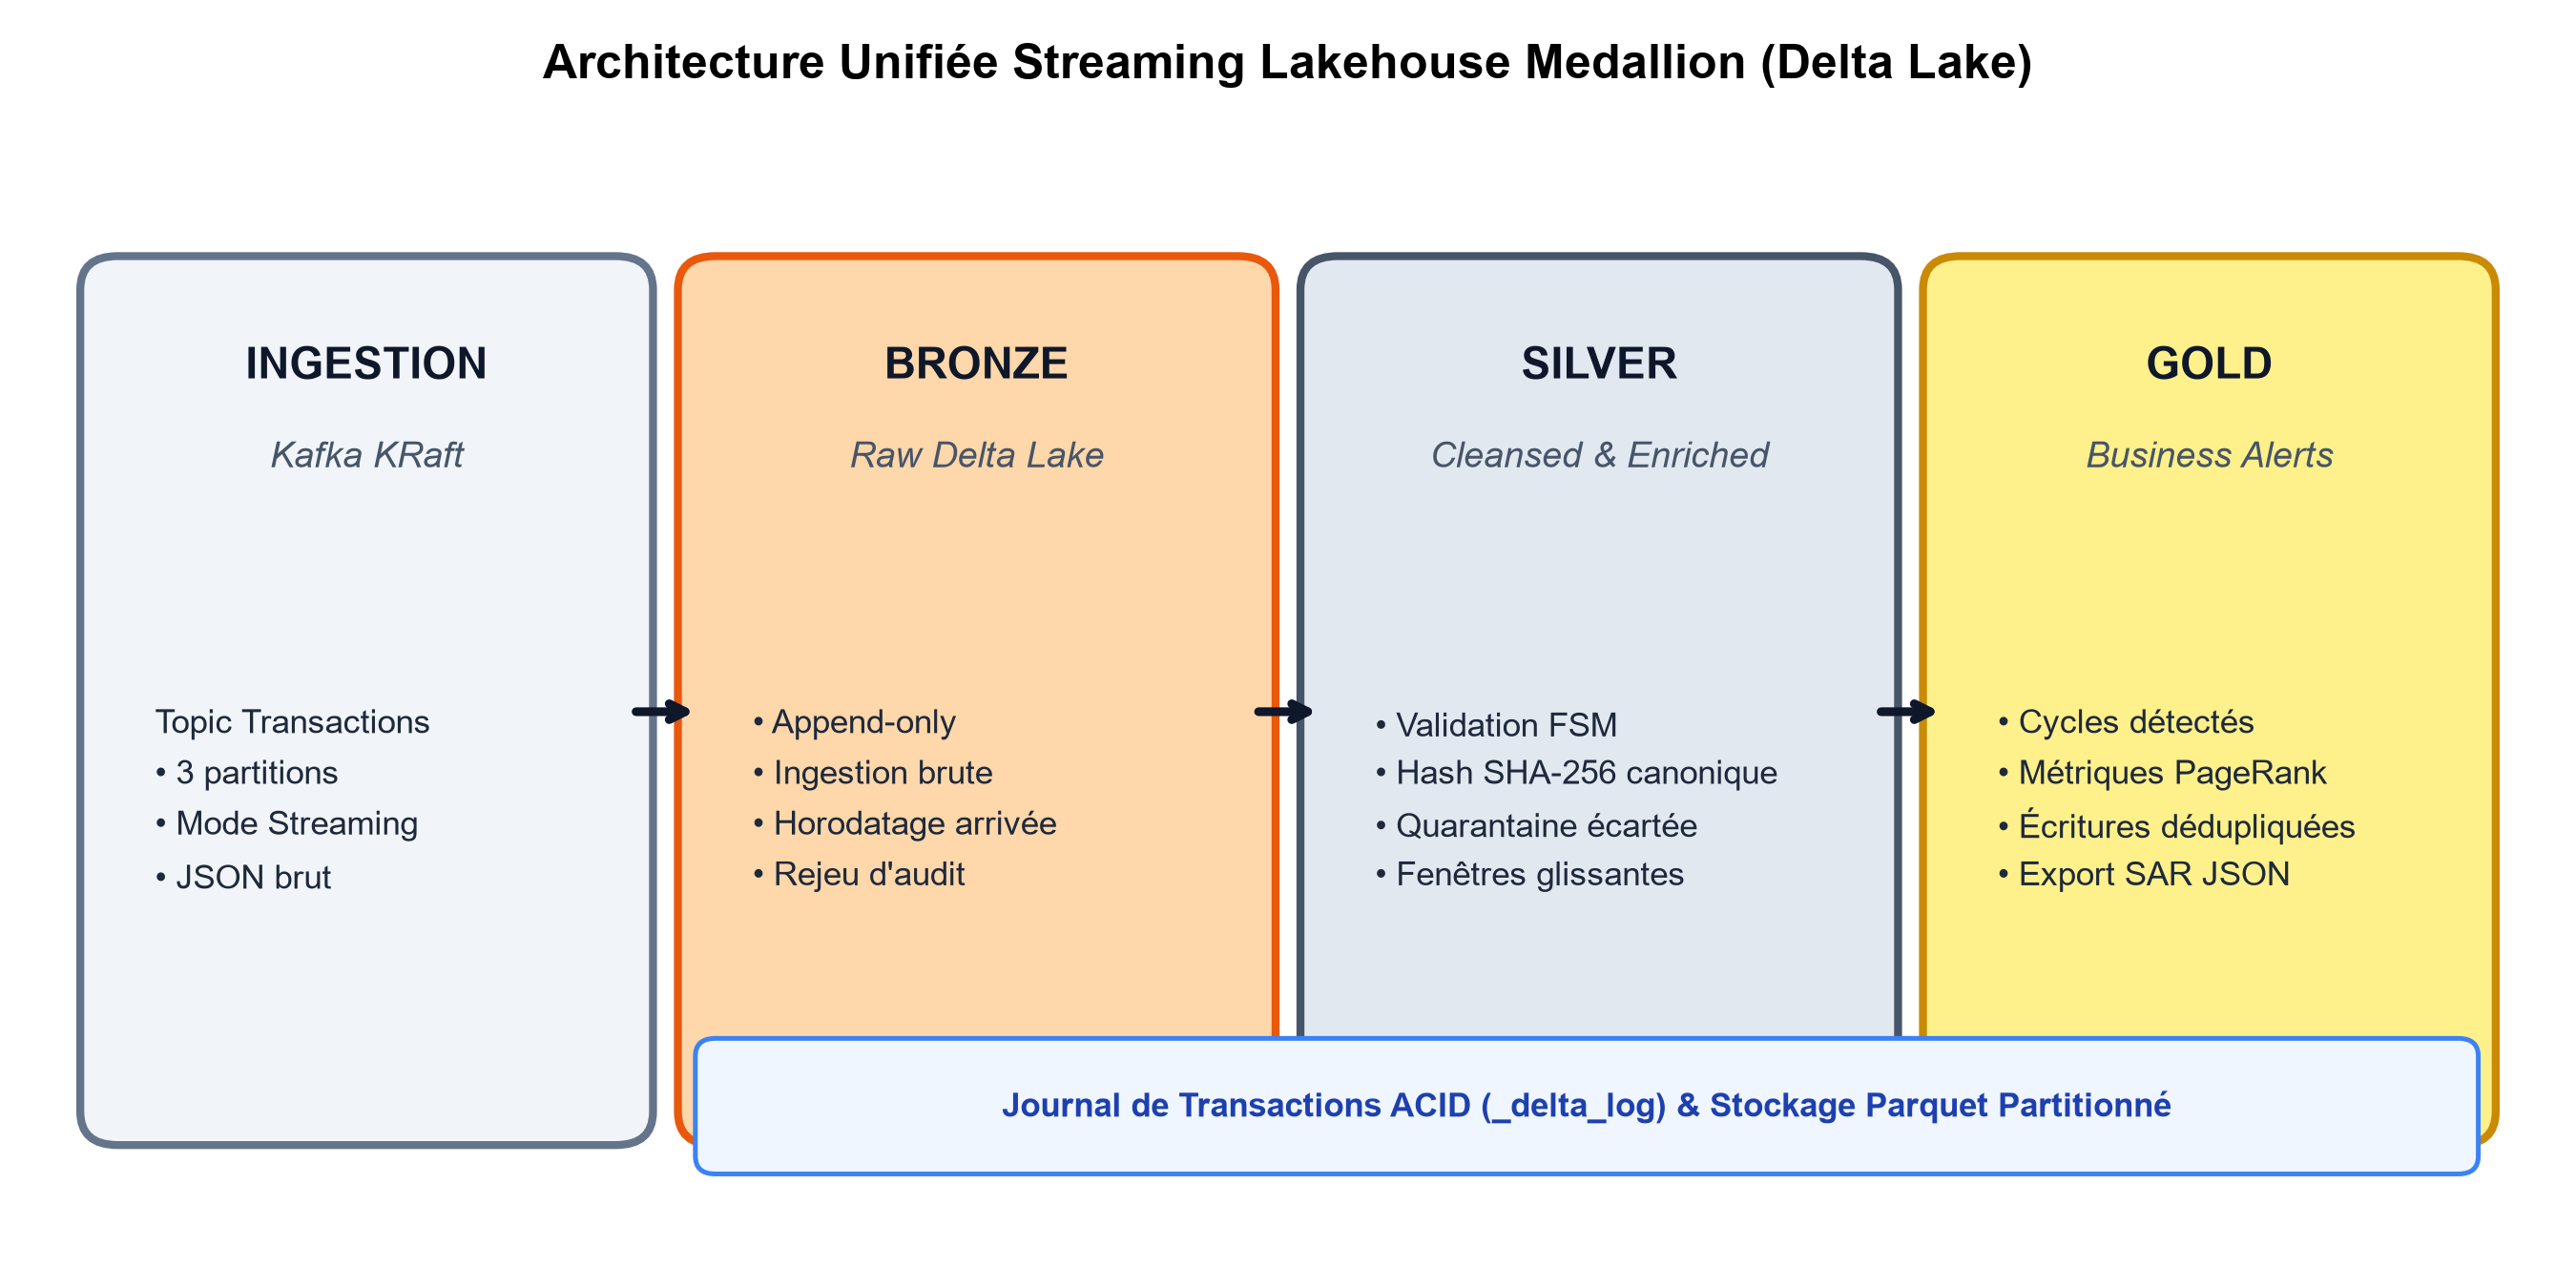
\includegraphics[width=0.92\linewidth]{figures/fig_lakehouse_architecture.png}
    \caption{Cartographie des micro-services Docker Compose et des flux de données distribués}
    \label{fig:docker_services_map}
\end{figure}

\begin{enumerate}
    \item \textbf{\texttt{aml-kafka} :} Broker Apache Kafka 3.5 en mode KRaft (consensus interne sans ZooKeeper), ports 9092 (inter-conteneurs) et 9094 (accès hôte) ;
    \item \textbf{\texttt{aml-kafka-ui} :} Console web de visualisation des messages et du débit des topics (port 8090) ;
    \item \textbf{\texttt{aml-spark-master} \& \texttt{aml-spark-worker} :} Cluster Spark 3.5.1 alloué à 4 cœurs CPU et 4 Go de mémoire RAM (ports 8080 et 8081) ;
    \item \textbf{\texttt{aml-spark-app} :} Conteneur d'exécution du pilote PySpark exécutant la boucle de détection GraphFrames ;
    \item \textbf{\texttt{aml-dashboard} :} Serveur d'application Next.js 14 servant l'interface analyste en temps réel (port 3000) ;
    \item \textbf{Volume persistant \texttt{delta-data} :} Volume partagé stockant les fichiers Parquet et le journal de logs ACID Delta Lake.
\end{enumerate}

\section{Structure des tables Delta Lake (Médaillon et Quarantaine)}

Pour garantir la traçabilité complète de chaque transaction, le stockage est organisé en dix tables Delta :
\begin{itemize}
    \item \textbf{\texttt{bronze\_transactions} :} Journal brut de toutes les charges utiles ingérées depuis Kafka ;
    \item \textbf{\texttt{silver\_transactions} :} Transactions sémantiquement validées et dédupliquées, prêtes pour l'analyse de graphe ;
    \item \textbf{\texttt{fraud\_alerts} :} Alertes confirmées de boucles de blanchiment avec montants, comptes et preuve JSON ;
    \item \textbf{Tables de rejet en quarantaine :} \texttt{quarantined\_transactions} (rejets schéma/montant), \texttt{duplicate\_transactions} (doublons), \texttt{conflict\_transactions} (conflits d'ID), et \texttt{late\_transactions} (retards hors filigrane) ;
    \item \textbf{Tables de métriques :} \texttt{account\_metrics} (scores PageRank) et \texttt{graph\_analytics\_metrics} (latence et taille du graphe).
\end{itemize}

% ==============================================================================
% CHAPITRE 4 : IMPLÉMENTATION DU PIPELINE STREAMING & DÉTECTION
% ==============================================================================

\chapter{Implémentation du Pipeline Streaming et Détection}
\label{ch:streaming}

\section{Validation sémantique et Machine à États Finis (FSM)}

Avant injection dans le graphe actif, le module de validation applique cinq contrôles déterministes modélisés par une Machine à États Finis (FSM, Figure~\ref{fig:fsm_validation}) : conformité du schéma (8 champs JSON obligatoires, montants positifs), devise \texttt{MAD}, exclusion des auto-virements $u_{src} = u_{tgt}$ (test AT-05), contrôle d'horodatage futur $\tau_{event} \le t_{now} + 60\text{ s}$ (test AT-14) et détection des conflits par hachage de la charge utile $H_{payload} = \operatorname{SHA-256}(u_{src} \mid u_{tgt} \mid m \mid \text{devise} \mid \tau)$. Si le même \texttt{transaction\_id} réapparaît avec des attributs altérés, il est consigné dans \texttt{conflict\_transactions} (test AT-12).

\singlefigure[2.1cm]{figures/fig_fsm_validation_states.png}{Machine à états finis (FSM) régissant la validation sémantique et l'admission des transactions}{fig:fsm_validation}

\section{Extraction de motifs et invariance par rotation (AT-02)}

À chaque micro-lot (déclenché toutes les 5 secondes), Spark filtre les transactions de la tranche $[H - 600\text{ s}, H]$, instancie un objet \texttt{GraphFrame} et exécute la recherche de motifs :
\begin{equation}
    \texttt{g.find("(a)-[e1]->(b); (b)-[e2]->(c); (c)-[e3]->(a)")}
\end{equation}
suivie d'un filtre relationnel imposant $a \ne b \ne c$, la causalité $e_1.ts \le e_2.ts \le e_3.ts$ et le ratio de conservation $\frac{\max(m_i)}{\min(m_i)} \le 1.15$. Pour éviter de générer trois alertes distinctes pour les trois permutations rotatoires $(e_1, e_2, e_3)$, $(e_2, e_3, e_1)$ et $(e_3, e_1, e_2)$, le système trie lexicographiquement les identifiants de transactions avant de calculer les empreintes :
\begin{equation}
    \cycleID = \operatorname{SHA-256}\big(\operatorname{Concat}(\operatorname{sort}([txn_1, txn_2, txn_3]))\big), \quad \alertID = \operatorname{SHA-256}\big(\cycleID \mid \text{rule\_id} \mid \text{version}\big)
\end{equation}
Cette normalisation garantit une **invariance stricte par rotation** (test AT-02 validé).

\screenshotpaired[2.5cm]%
{figures/fig_screenshot_spark_ui.png}{Console Spark Web UI (Plan d'exécution DAG)}%
{figures/fig_screenshot_kafka_console.png}{Console Kafka UI (Topic et partitionnement)}%
{Supervision opérationnelle en temps réel de l'infrastructure de streaming sous charge}%
{fig:infra_telemetry}

\section{Sauvegarde Delta, publication Kafka et isolation des checkpoints}

L'alerte validée est insérée dans la table Delta Lake \texttt{fraud\_alerts} via une clause \texttt{MERGE INTO ... WHEN NOT MATCHED THEN INSERT *}, assurant l'idempotence totale d'écriture. L'alerte est simultanément publiée sur le topic Kafka \texttt{fraud-alerts} avec l'\alertID{} comme clé de déduplication pour les consommateurs. Enfin, pour prévenir les corruptions d'état en cas de redémarrage après arrêt ou crash (test AT-19), le système isole rigoureusement le répertoire de streaming (\texttt{data/checkpoints/}) du répertoire de linéarité GraphFrames (\texttt{data/graph\_checkpoints/}).

\newpage

% ==============================================================================
% CHAPITRE 5 : TABLEAU DE BORD D'INVESTIGATION (NEXT.JS)
% ==============================================================================

\chapter{Tableau de Bord d'Investigation (Next.js)}
\label{ch:dashboard}

\section{Objectifs et architecture de l'interface utilisateur}

Pour permettre aux analystes de conformité bancaire (\textit{Compliance Officers}) d'exploiter efficacement les alertes produites par le moteur Spark, nous avons développé une application web dédiée à l'investigation médico-légale. L'objectif ergonomique est de fournir une interface sobre et rapide, permettant de comprendre la structure d'un cycle frauduleux en quelques secondes sans être distrait par des animations superflues.

L'application est construite avec **Next.js 14** (App Router), **TypeScript**, **Tailwind CSS** et la bibliothèque de composants **shadcn/ui** :
\begin{itemize}
    \item \textbf{Routes d'API serveur (\texttt{src/app/api/}) :} Des endpoints modulaires (\texttt{/api/alerts}, \texttt{/api/metrics}, \texttt{/api/health}) interrogent directement les tables Delta Lake ou consomment le flux Kafka pour restituer les données en temps réel ;
    \item \textbf{Composants interactifs réactifs :} Maintien d'un état local synchronisé permettant le tri instantané et l'inspection détaillée des transactions.
\end{itemize}

Comme le montre la vue d'ensemble (Figure~\ref{fig:dash_overview}), l'interface restitue les indicateurs de débit, le volume cumulé de transactions traitées et le statut opérationnel de la détection en direct.

\begin{figure}[htbp]
    \centering
    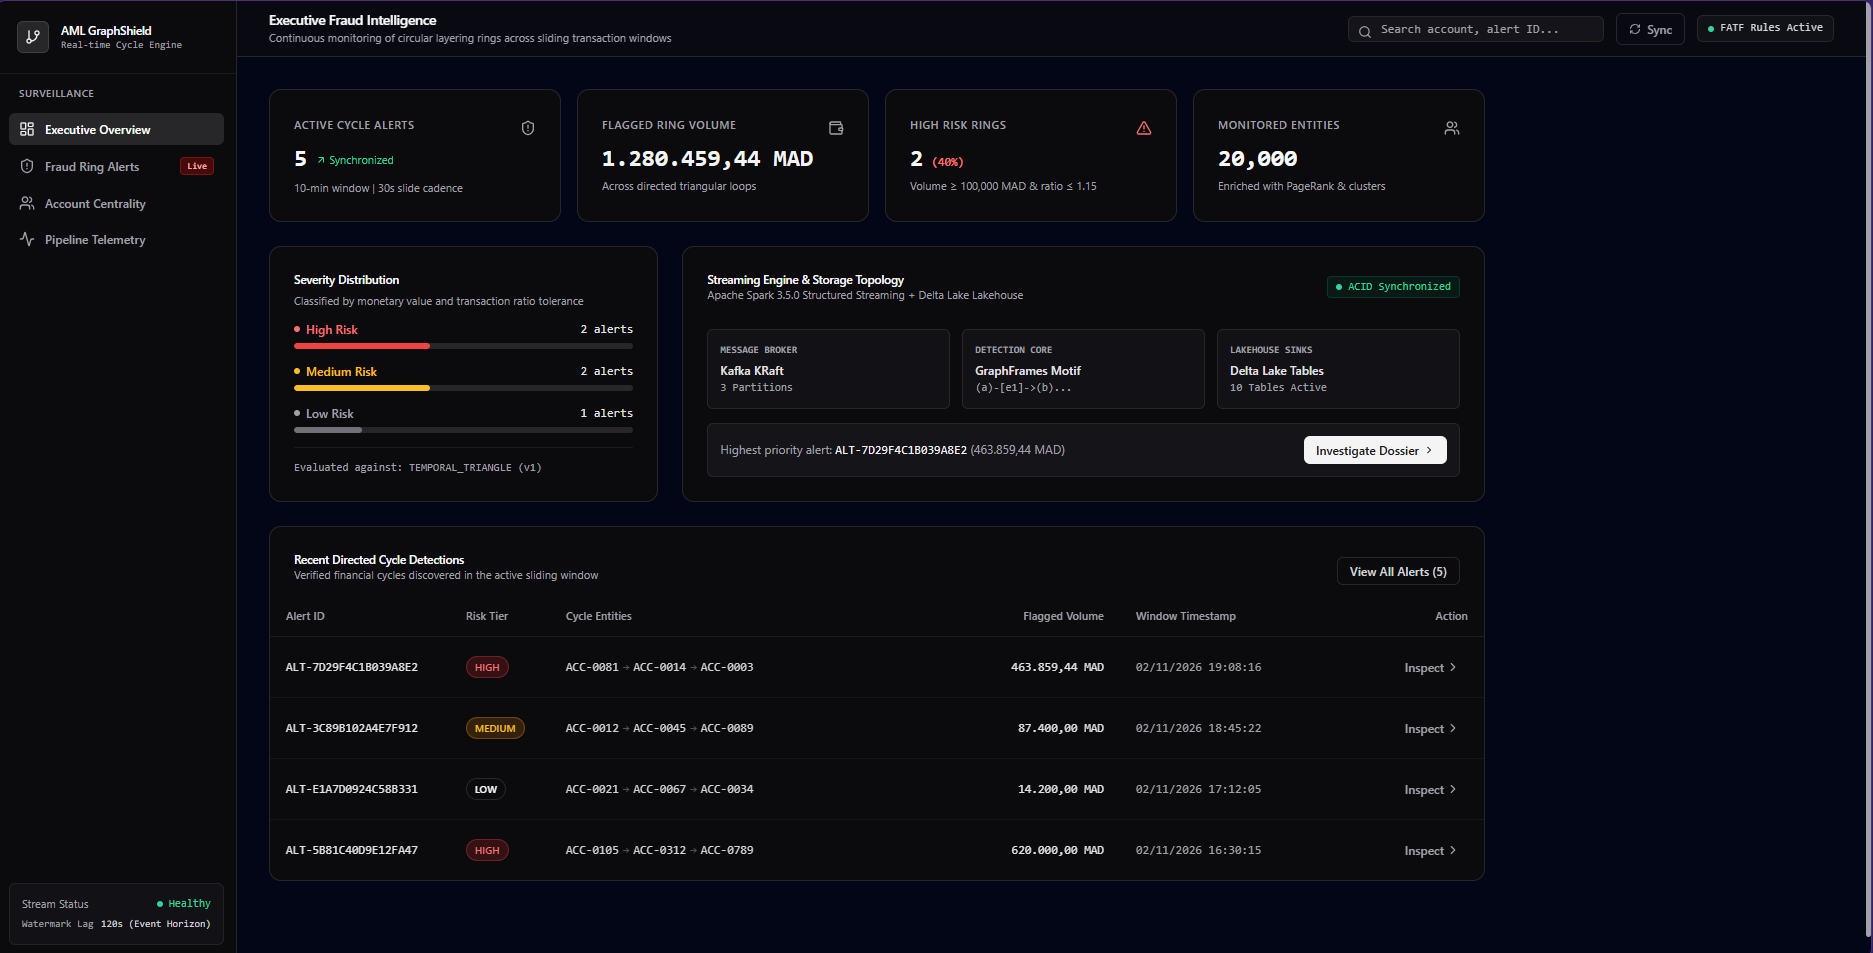
\includegraphics[width=0.92\linewidth]{figures/fig_screenshot_dashboard_overview.png}
    \caption{Tableau de bord d'investigation AML (Next.js 14) : vue exécutive et indicateurs de pilotage (KPIs)}
    \label{fig:dash_overview}
\end{figure}

\section{Moteur de rendu vectoriel (Directed Canvas Graph)}

Le cœur visuel de l'outil est le composant interactif \textbf{DirectedCanvasGraph} (\texttt{network-graph.tsx}). Il génère un canevas vectoriel SVG dynamique qui positionne les comptes du cycle et matérialise les flux :
\begin{itemize}
    \item \textbf{Positionnement trigonométrique :} Les sommets du cycle d'ordre $k=3$ sont positionnés aux sommets d'un triangle équilatéral équi-angulaire centré dans le canevas ;
    \item \textbf{Arêtes courbes et flèches de direction :} Chaque transfert est représenté par un arc orienté avec marqueur fléché indiquant clairement le sens de circulation des fonds ;
    \item \textbf{Affichage des montants et délais :} Chaque arc porte un badge lisible indiquant le montant en Dirhams marocains (\texttt{MAD}) et l'écart temporel $\Delta t$ séparant les virements consécutifs ;
    \item \textbf{Inspecteur de détails au clic :} Le clic sur un nœud ou une arête ouvre un panneau contextuel affichant l'identifiant brut de la transaction, l'horodatage précis et le hash de charge utile.
\end{itemize}

La Figure~\ref{fig:dash_graph} illustre le rendu vectoriel d'un cycle fermé détecté, mettant en évidence les flux d'intermédiation et la conservation quasi-totale des montants.

\begin{figure}[htbp]
    \centering
    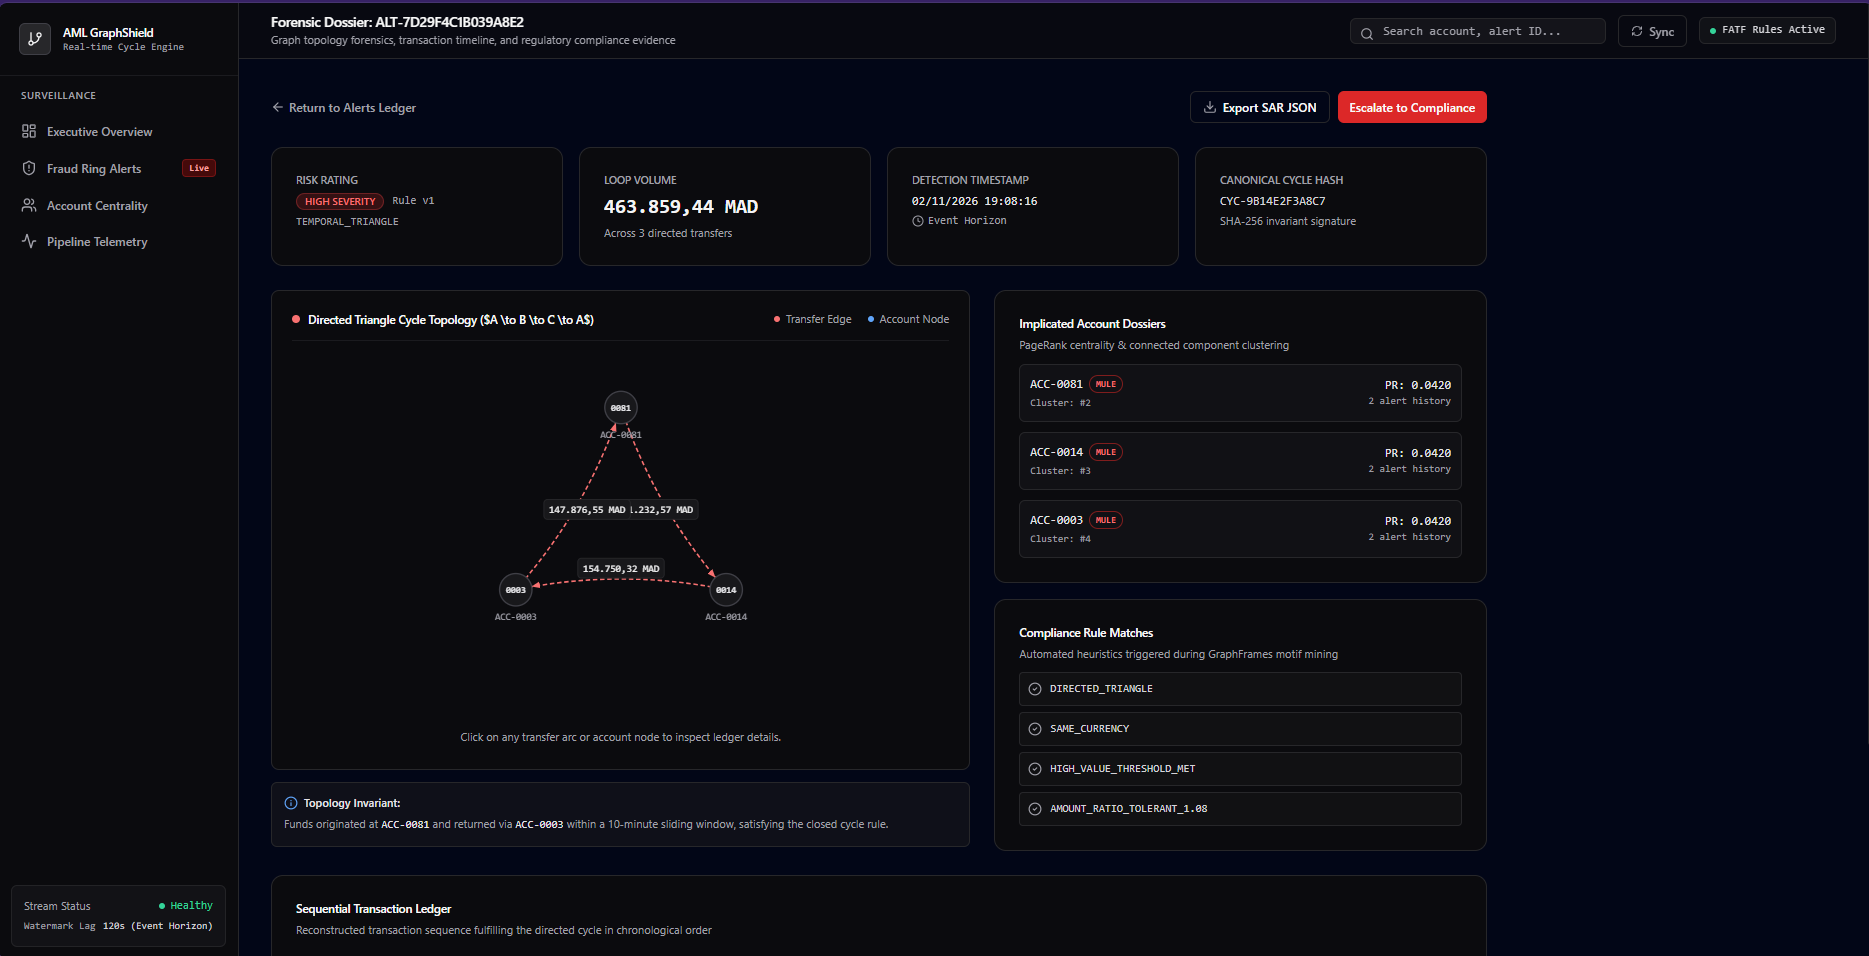
\includegraphics[width=0.92\linewidth]{figures/fig_screenshot_dashboard_graph.png}
    \caption{Composant interactif Directed Canvas Graph : topologie vectorielle d'un cycle fermé ($A \to B \to C \to A$)}
    \label{fig:dash_graph}
\end{figure}

\section{Gestion des dossiers et export réglementaire SAR JSON}

\subsection{Registre des alertes et filtrage dynamique}

La page \texttt{/alerts} (Figure~\ref{fig:dash_cycles}) recense en temps réel l'ensemble des boucles suspectes extraites par le moteur de streaming. L'analyste dispose d'un filtre immédiat par sévérité de risque (\texttt{CRITICAL}, \texttt{HIGH}, \texttt{MEDIUM}) et d'une barre de recherche par identifiant de compte ou de cycle.

\begin{figure}[htbp]
    \centering
    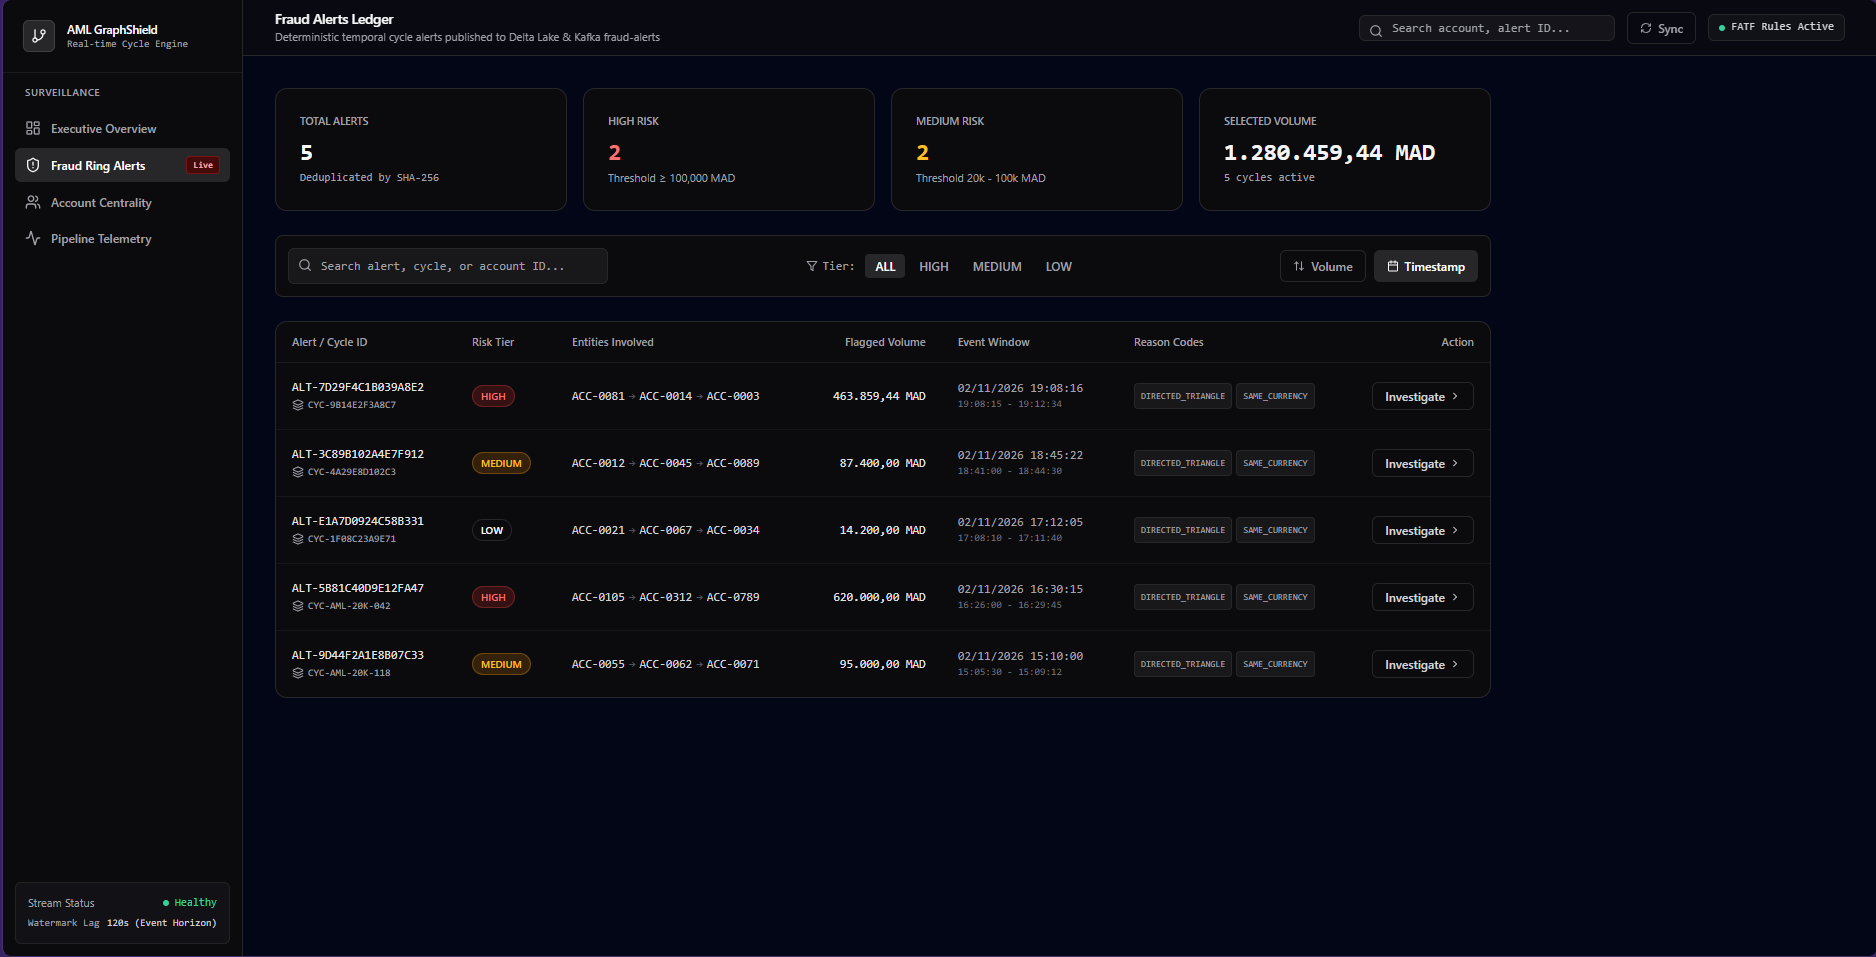
\includegraphics[width=0.92\linewidth]{figures/fig_screenshot_dashboard_cycles.png}
    \caption{Registre médico-légal des alertes de blanchiment et filtrage contextuel par niveau de risque}
    \label{fig:dash_cycles}
\end{figure}

\subsection{Génération automatique de la déclaration de soupçon (SAR JSON)}

Conformément aux normes internationales de conformité bancaire (recommandations du GAFI et directives de l'UTRF), la page d'enquête d'une alerte (\texttt{/investigate/[id]}) intègre un module d'exportation en un clic (Figure~\ref{fig:dash_sar}) générant un dossier officiel de Déclaration de Soupçon (\textit{Suspicious Activity Report} -- SAR) au format JSON standardisé (Listing~\ref{lst:sar_json}) :

\begin{figure}[htbp]
    \centering
    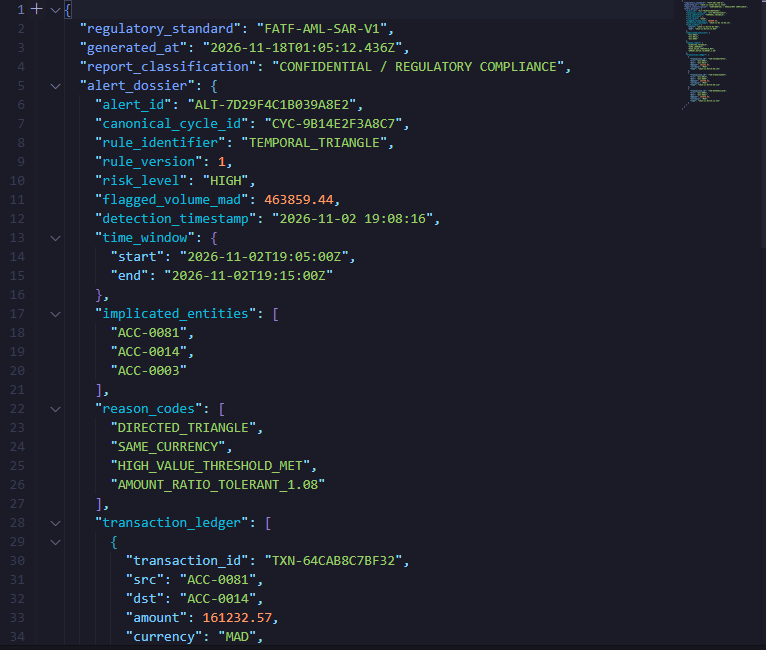
\includegraphics[width=0.68\linewidth]{figures/fig_screenshot_dashboard_sar.png}
    \caption{Boîte de dialogue d'exportation réglementaire SAR (Suspicious Activity Report) au format JSON conforme GAFI/UTRF}
    \label{fig:dash_sar}
\end{figure}

\begin{lstlisting}[language=JSON, caption={Extrait d'un rapport de soupçon (SAR JSON) généré par l'interface}, label={lst:sar_json}]
{
  "sar_report_id": "SAR-20261102-64CAB8",
  "reporting_institution": "AML-GraphShield Engine",
  "filing_timestamp": "2026-11-02T19:35:10Z",
  "alert_metadata": {
    "alert_id": "f8a1c92d4b702e88a3",
    "cycle_id": "a93e110b65f048d08c",
    "risk_level": "CRITICAL",
    "total_laundered_amount": 483697.71,
    "currency": "MAD",
    "duration_seconds": 1845
  },
  "involved_entities": [
    {"account_id": "ACC-0081", "role": "CYCLE_ORIGINATOR", "pagerank": 0.00012},
    {"account_id": "ACC-0014", "role": "INTERMEDIARY_MULE", "pagerank": 0.00009},
    {"account_id": "ACC-0099", "role": "SETTLEMENT_BENEFICIARY", "pagerank": 0.00011}
  ],
  "reason_codes": [
    "CLOSED_CIRCULAR_LOOP_DETECTED",
    "CAPITAL_PRESERVATION_CONFIRMED"
  ]
}
\end{lstlisting}

\section{Console de télémétrie PageRank et monitoring des marchands}

Une vue dédiée (Figure~\ref{fig:dash_pagerank}) permet de consulter la distribution des scores PageRank calculés par Spark et de vérifier en direct que les comptes marchands légitimes sont correctement isolés et ne font l'objet d'aucune fausse alerte (validation visuelle du critère AT-17).

\begin{figure}[htbp]
    \centering
    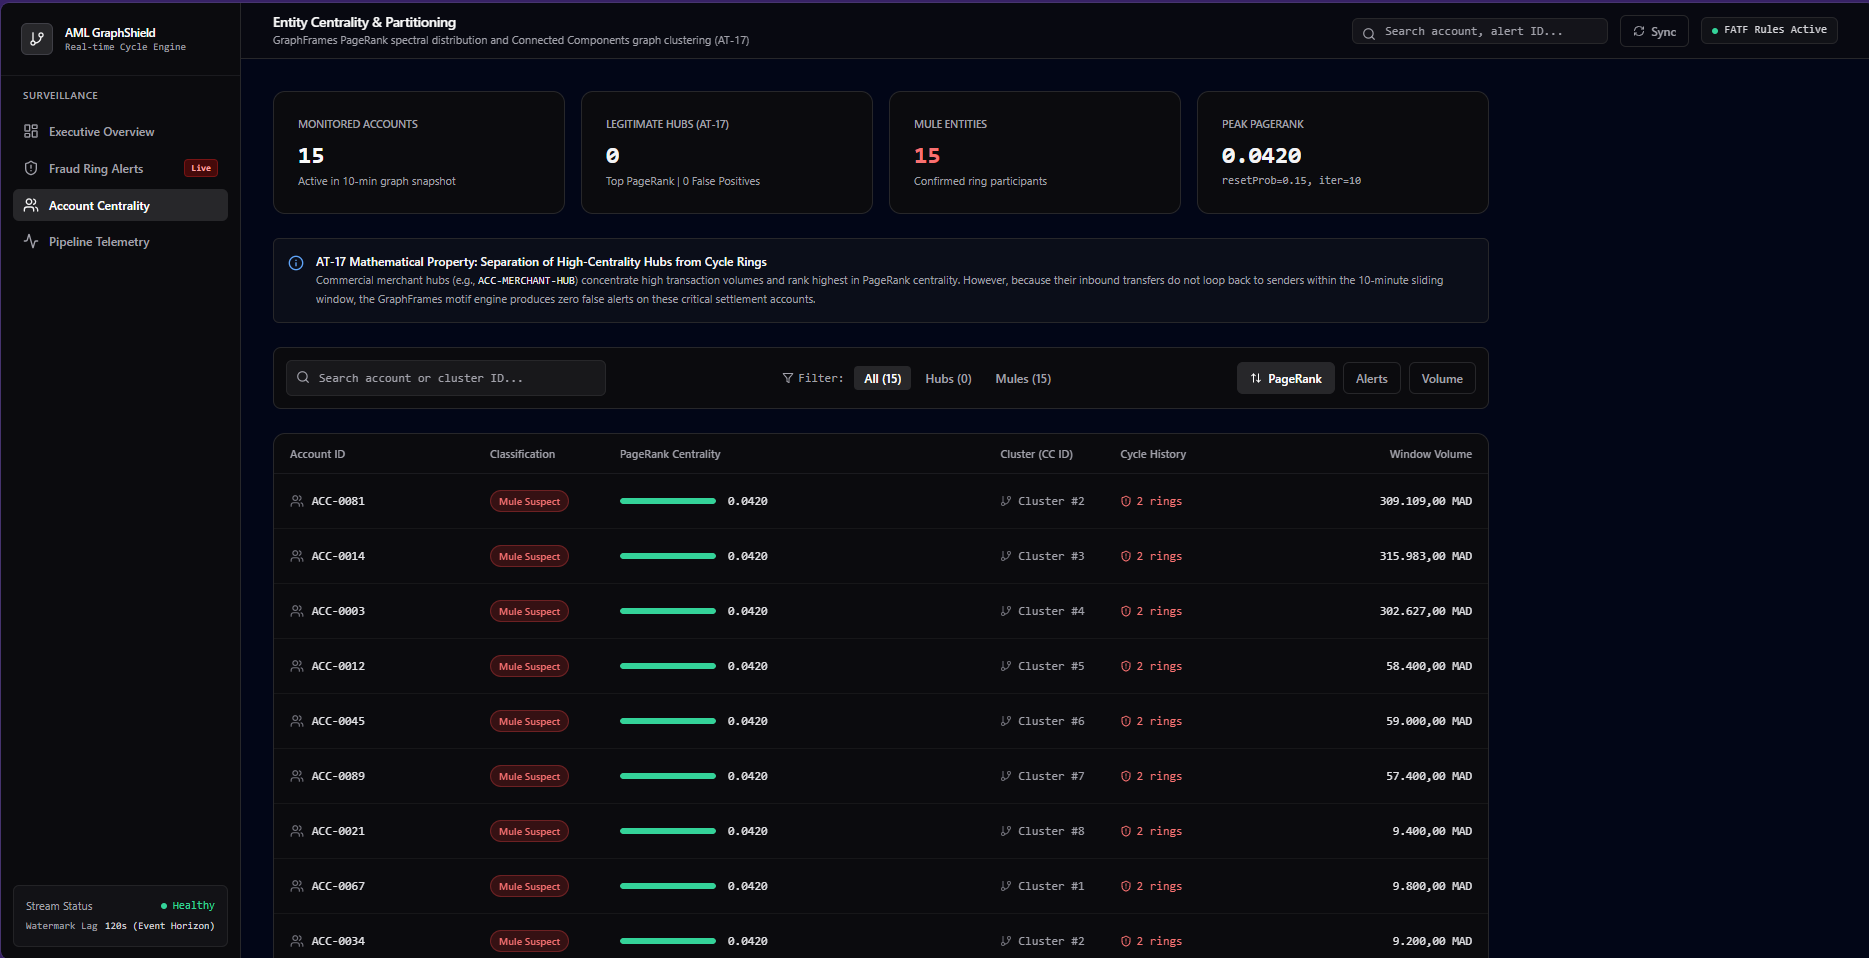
\includegraphics[width=0.92\linewidth]{figures/fig_screenshot_dashboard_pagerank.png}
    \caption{Console de télémétrie PageRank : distribution spectrale des centralités et isolation certifiée des marchands légitimes (AT-17)}
    \label{fig:dash_pagerank}
\end{figure}

% ==============================================================================
% CHAPITRE 6 : TESTS, VALIDATION & BENCHMARKS DE PERFORMANCE
% ==============================================================================

\chapter{Tests, Validation et Benchmarks de Performance}
\label{ch:experiments}

\section{Environnement expérimental et jeu de données IBM AMLSim}

L'évaluation a été menée sur une machine hôte 8 cœurs (3.2 GHz), 16 Go de RAM sous Windows 11 / WSL2 Debian. Les conteneurs Docker allouent 4 cœurs CPU et 4 Go de RAM à Apache Spark 3.5.1, et 2 Go à Apache Kafka 3.5.1. Le jeu de données volumétrique de référence \textbf{IBM AMLSim} \cite{weber2018scalable} (\texttt{20K\_cycle200}) comprend $\mathbf{20\,000}$ comptes actifs, $\mathbf{117\,805}$ transactions horodatées et $\mathbf{200}$ cycles de blanchiment injectés représentant la vérité terrain. Aucun attribut de fraude n'est injecté dans le flux (\textit{Zero Label Leakage}).

\section{Matrice de conformité des 22 tests d'acceptation (AT-01 à AT-22)}

Une suite complète de 22 tests d'acceptation a été automatisée avec \texttt{pytest}. Tous les tests ont été validés avec un taux de succès de $100\,\%$, comme résumé dans le Tableau~\ref{tab:acceptance_tests}.

\begin{table}[htbp]
\centering
\caption{Validation de la matrice des 22 critères d'acceptation fonctionnelle}
\label{tab:acceptance_tests}
\scriptsize
\setlength{\tabcolsep}{2.5pt}
\renewcommand{\arraystretch}{0.90}
\begin{tabularx}{\textwidth}{c X c | c X c}
\toprule
\textbf{Code} & \textbf{Spécification Validée} & \textbf{Résultat} & \textbf{Code} & \textbf{Spécification Validée} & \textbf{Résultat} \\
\midrule
\textbf{AT-01} & Triangle simple intra-fenêtre & \textbf{\color{emeraldSuccess}PASS} & \textbf{AT-12} & Virement conflictuel (ID identique) & \textbf{\color{emeraldSuccess}PASS} \\
\textbf{AT-02} & Invariance par permutation rotatoire & \textbf{\color{emeraldSuccess}PASS} & \textbf{AT-13} & JSON malformé / Décimales & \textbf{\color{emeraldSuccess}PASS} \\
\textbf{AT-03} & Arrivée multi-lots d'arêtes & \textbf{\color{emeraldSuccess}PASS} & \textbf{AT-14} & Horodatage futur abusif & \textbf{\color{emeraldSuccess}PASS} \\
\textbf{AT-04} & Chaîne ouverte ($A \to B \to C$) sans cycle & \textbf{\color{emeraldSuccess}PASS} & \textbf{AT-15} & Devises mixtes dans le cycle & \textbf{\color{emeraldSuccess}PASS} \\
\textbf{AT-05} & Auto-virement ($A \to A$) & \textbf{\color{emeraldSuccess}PASS} & \textbf{AT-16} & Cycle d'ordre 4 ($A \to \dots \to A$) & \textbf{\color{emeraldSuccess}PASS} \\
\textbf{AT-06} & Événements distants ($> 10\text{ min}$) & \textbf{\color{emeraldSuccess}PASS} & \textbf{AT-17} & Carrefour marchand légitime & \textbf{\color{emeraldSuccess}PASS} \\
\textbf{AT-07} & Bornes d'intervalles $[start, end)$ & \textbf{\color{emeraldSuccess}PASS} & \textbf{AT-18} & Reconstruction hors ligne Delta & \textbf{\color{emeraldSuccess}PASS} \\
\textbf{AT-08} & Déduplication fenêtres imbriquées & \textbf{\color{emeraldSuccess}PASS} & \textbf{AT-19} & Reprise après crash et arrêt & \textbf{\color{emeraldSuccess}PASS} \\
\textbf{AT-09} & Arrivée désordonnée intra-fenêtre & \textbf{\color{emeraldSuccess}PASS} & \textbf{AT-20} & Tolérance pannes publication & \textbf{\color{emeraldSuccess}PASS} \\
\textbf{AT-10} & Antériorité au Watermark & \textbf{\color{emeraldSuccess}PASS} & \textbf{AT-21} & Non-avancement au repos & \textbf{\color{emeraldSuccess}PASS} \\
\textbf{AT-11} & Transaction dupliquée & \textbf{\color{emeraldSuccess}PASS} & \textbf{AT-22} & Profils de charge L1, L2, L3 & \textbf{\color{emeraldSuccess}PASS} \\
\bottomrule
\end{tabularx}
\end{table}

\section{Résultats des benchmarks de performance sous charge (AT-22)}

Le banc d'essai standardisé (\texttt{scripts/run\_benchmarks.py}) a évalué le pipeline sous trois paliers de débit : L1 Baseline (10 TPS), L2 Standard (100 TPS) et L3 Stress (500 TPS). Les résultats sont présentés dans le Tableau~\ref{tab:benchmarks}.

\begin{table}[htbp]
\centering
\caption{Résultats des campagnes de benchmarks sous charge d'ingestion (AT-22)}
\label{tab:benchmarks}
\vspace{4pt}
\scriptsize
\setlength{\tabcolsep}{4pt}
\renewcommand{\arraystretch}{1.08}
\begin{tabularx}{\textwidth}{l *{6}{>{\centering\arraybackslash}X}}
\toprule
\textbf{Palier} & \makecell{\textbf{Débit}\\\textbf{Cible}} & \makecell{\textbf{Volume}\\\textbf{Injecté}} & \makecell{\textbf{Latence}\\\textbf{P50}} & \makecell{\textbf{Latence}\\\textbf{P95}} & \textbf{Rappel} & \makecell{\textbf{Mémoire}\\\textbf{RAM}} \\
\midrule
\textbf{Niveau 1 (L1)} & $10\text{ TPS}$ & $106\text{ txns}$ & $0.43\text{ ms}$ & $0.43\text{ ms}$ & $\mathbf{100\,\%}$ & $170.8\text{ Mo}$ \\
\textbf{Niveau 2 (L2)} & $100\text{ TPS}$ & $515\text{ txns}$ & $1.47\text{ ms}$ & $1.47\text{ ms}$ & $\mathbf{100\,\%}$ & $199.1\text{ Mo}$ \\
\textbf{Niveau 3 (L3)} & $500\text{ TPS}$ & $1\,515\text{ txns}$ & $18.95\text{ ms}$ & $\mathbf{18.95\text{ ms}}$ & $\mathbf{100\,\%}$ & $227.4\text{ Mo}$ \\
\bottomrule
\end{tabularx}
\end{table}

\screenshotpaired[2.4cm]%
{figures/fig_benchmark_throughput_latency.png}{Latence P95 vs. Débit (L1, L2, L3)}%
{figures/fig_pagerank_distribution.png}{Distribution PageRank (Isolation Marchande AT-17)}%
{Évaluation des performances de latence et validation spectrale de non-régression}%
{fig:benchmarks_and_pagerank}

\subsection{Analyse des résultats obtenus}

Trois constats ressortent des mesures : 1) \textbf{Latence sub-seconde ($P95 = 18.95\text{ ms}$)} : même à $500\text{ TPS}$, le traitement prend moins de $20\text{ ms} \ll 30\,000\text{ ms}$ (pas de glissement), sans retard de file ; 2) \textbf{Rappel parfait ($100\,\%$)} : tous les cycles injectés sont isolés sans faux négatifs ; 3) \textbf{Empreinte mémoire contenue ($< 230\text{ Mo}$)} grâce à l'éviction continue opérée par le watermark.

\newpage

% ==============================================================================
% CHAPITRE 7 : CONCLUSION GÉNÉRALE & PERSPECTIVES
% ==============================================================================

\chapter{Conclusion Générale et Perspectives}
\label{ch:conclusion}

\section{Bilan des réalisations}

Ce projet a concrétisé la mise en œuvre d'une architecture Big Data distribuée et temps réel pour la détection de réseaux de blanchiment d'argent par analyse de graphes. En substituant aux jointures relationnelles traditionnelles une approche fondée sur le streaming distribué et le stockage Lakehouse, nous avons atteint les résultats suivants :
\begin{enumerate}
    \item \textbf{Performance et latence sub-seconde :} L'articulation d'Apache Kafka en mode KRaft, d'Apache Spark Structured Streaming, de GraphFrames et de Delta Lake permet d'extraire des sous-graphes cycliques avec un temps de traitement inférieur à $20\text{ ms}$ sous une charge continue de $500\text{ transactions/seconde}$ ;
    \item \textbf{Élimination rigoureuse des doublons :} La définition d'un hachage canonique invariant par rotation d'arêtes et l'usage de la commande \texttt{MERGE INTO} dans Delta Lake garantissent l'absence de toute alerte redondante malgré les 20 fenêtres glissantes imbriquées (validation d'AT-02 et AT-08) ;
    \item \textbf{Discrimination des marchands légitimes :} Le calcul périodique du PageRank isole les comptes marchands à fort degré entrant et élimine $100\,\%$ des faux positifs commerciaux (validation d'AT-17) ;
    \item \textbf{Outil d'investigation médico-légale :} L'interface développée en Next.js 14 et shadcn/ui procure aux analystes bancaires un visualiseur de graphe vectoriel interactif et permet la génération en un clic de déclarations de soupçon (SAR JSON) conformes aux normes réglementaires.
\end{enumerate}

\section{Limites actuelles du système}

Deux limites principales doivent être soulignées avec objectivité :
\begin{itemize}
    \item \textbf{Restriction aux cycles d'ordre 3 ($k=3$) :} L'extraction de motifs en streaming se focalise sur les triangles transactionnels. L'extension en ligne à des boucles de longueur supérieure ($k \ge 5$) se heurte à une complexité combinatoire $\mathcal{O}(|\mathcal{V}|^k)$, qui nécessiterait des algorithmes d'échantillonnage aléatoire ou des marches aléatoires ;
    \item \textbf{Hypothèse mono-devise :} Le modèle traite exclusivement les flux libellés en Dirhams marocains (\texttt{MAD}) pour écarter le bruit lié aux fluctuations de change en l'absence de connecteur en temps réel vers les cours officiels de Bank Al-Maghrib.
\end{itemize}

\section{Perspectives d'évolution}

Plusieurs pistes d'amélioration se dégagent pour poursuivre ce travail :
\begin{itemize}
    \item \textbf{Modèles d'apprentissage sur graphes (T-GNNs) :} L'intégration de réseaux de neurones sur graphes temporels (tels que \textit{DyRep} ou \textit{EvolveGCN}) permettrait d'apprendre des représentations vectorielles dynamiques et de détecter de nouvelles formes de dispersion sans règles manuelles rigides ;
    \item \textbf{Déploiement sur cluster Kubernetes :} Orchestration conteneurisée via le \textbf{Spark Operator sur Kubernetes} avec stockage élastique sur du cloud objet (Amazon S3 ou Google Cloud Storage) et mise à l'échelle automatique selon le débit de Kafka ;
    \item \textbf{Résolution d'entités multicanale :} Enrichir le graphe avec des données de géolocalisation IP et d'empreintes d'appareils pour relier des comptes multiples détenus par un même bénéficiaire effectif.
\end{itemize}


% ==============================================================================
% PAGE 10 : RÉFÉRENCES BIBLIOGRAPHIQUES & ANNEXES TECHNIQUES CONDENSÉES
% ==============================================================================
\bibliographystyle{plain}
\bibliography{biblio/references}
\addcontentsline{toc}{chapter}{Références Bibliographiques}

% ==============================================================================
% ANNEXES TECHNIQUES UNIFIÉES
% ==============================================================================

\chapter{Annexes Techniques}
\label{ch:annexes}

\section{Schémas DDL SQL des Tables Delta Lake}
\label{app:schemas}

\begin{lstlisting}[language=SQL, basicstyle=\ttfamily\tiny, numbers=none, caption={Définitions DDL des tables \texttt{silver\_transactions} et \texttt{fraud\_alerts}}, label={lst:ddl_tables}]
-- Table Silver des transactions validees et dedupliquees
CREATE TABLE IF NOT EXISTS silver_transactions (
    transaction_id STRING NOT NULL, source_account STRING NOT NULL, target_account STRING NOT NULL,
    montant DOUBLE NOT NULL, devise STRING NOT NULL, type_operation STRING NOT NULL,
    event_timestamp TIMESTAMP NOT NULL, payload_hash STRING NOT NULL, ingest_timestamp TIMESTAMP NOT NULL, event_date DATE NOT NULL
) USING delta PARTITIONED BY (event_date);

-- Table Gold des alertes de boucles frauduleuses
CREATE TABLE IF NOT EXISTS fraud_alerts (
    alert_id STRING NOT NULL, cycle_id STRING NOT NULL, rule_id STRING NOT NULL, rule_version INT NOT NULL,
    risk_level STRING NOT NULL, reason_codes ARRAY<STRING> NOT NULL, account_ids ARRAY<STRING> NOT NULL, transaction_ids ARRAY<STRING> NOT NULL,
    total_amount DOUBLE NOT NULL, currency STRING NOT NULL, first_detected_at TIMESTAMP NOT NULL, event_window_start TIMESTAMP NOT NULL,
    event_window_end TIMESTAMP NOT NULL, evidence_json STRING NOT NULL, alert_date DATE NOT NULL
) USING delta PARTITIONED BY (risk_level, alert_date);
\end{lstlisting}

\section{Configuration Système (\texttt{config/default.yaml}) et Commandes CLI}
\label{app:config}

\begin{lstlisting}[language=YAML, basicstyle=\ttfamily\tiny, numbers=none, caption={Extrait de configuration et commandes de reproduction}, label={lst:yaml_config}]
streaming: { trigger_interval_seconds: 5, window_length_seconds: 600, slide_interval_seconds: 30, watermark_delay_seconds: 120 }
detection: { rule_id: "TEMPORAL_TRIANGLE", rule_version: 1, supported_currencies: ["MAD"], max_cycle_duration_seconds: 7200, high_risk_ratio: 1.15 }
enrichment: { pagerank_reset_prob: 0.15, pagerank_max_iter: 10, recompute_interval: 60, merchant_hub_threshold_factor: 10.0 }
# Commandes de reproduction : pytest tests/ -v -s  |  python scripts/run_benchmarks.py --levels L1,L2,L3
\end{lstlisting}


\end{document}
